\documentclass{article}
\usepackage[utf8]{inputenc}
\usepackage{geometry}
\geometry{margin=1in}
\usepackage{amsmath}
\usepackage{amssymb}
\usepackage[ruled,vlined, linesnumbered]{algorithm2e}
\usepackage[english]{babel}
\usepackage[nottoc]{tocbibind}
\usepackage{color}
\usepackage{natbib}
\usepackage{graphicx}
\newtheorem{theorem}{Theorem}[section]

% Custom commands / shortcuts
\providecommand{\sign}{\textrm{sign}}
\providecommand{\note}[1]{\textcolor{red}{#1}}
\providecommand{\lam}{\lambda}

\title{Efficient Feature Screening for Lasso-Type
Problems via Batched Safe-Strong Rules}
\author{Chuyi Wang\\Department of Statistics and Actuarial Sciences\\University of Iowa
  \and
  Patrick Breheny\\Department of Biostatistics\\University of Iowa}
\date{}

\begin{document}

\maketitle

\section{Introduction}

The lasso (least absolute shrinkage and selection operator) model\citep{tibshirani1996regression}, is a popular model in statistics and machine learning, especially in high-dimensional problems. The model can be defined as the following modification of the least squares optimization problem:
\begin{equation}
    \hat{\beta}(\lambda)=\underset{\beta\in \mathbb{R}^p}{\mathrm{argmin}}\frac{1}{2n}||y-X\beta||_2^2+\lambda||\beta||_1,
\end{equation}
where $y$ is the $n\times 1$ response vector correspond to $n$ observations, $X=(x_1,x_2,...,x_p)$ is the $n\times p$ feature matrix correspond to $p$ features, $\beta\in \mathbb{R}^p$ is the $p\times 1$ coefficient vector and $\lambda$ is the regularization tuning parameter. $||\cdot||_2$ denotes the $l_2$ (Euclidean) norm and $||\cdot||_1$ denotes the $l_1$ norm. 

The lasso model has several attractive properties compared to least squares regression, including increased stability of estimation, increased prediction accuracy, and automatic variable selection arising from the fact that it yields sparse estimates of $\beta$.  As a result, it is widely applied in different fields, such as gene expression data analysis, image recognition and text mining, and has been extended in several ways, such as group lasso\cite{yuan2006model}, elastic net\cite{zou2005regularization} and sparse generalized linear models. Because of its wide popularity, solving the lasso model efficiently is an important topic in statistics and machine learning.

Because the optimal value of $\lambda$ is not known in advance, typical practice is to solve for $\beta$ along a sequence of values of the tuning parameter $\lambda$, known as the solution path.  Pathwise algorithms can be efficiently implemented by using the solution at a previous $\lambda$ value as a ``warm start'' for the next value of $\lambda$.  In particular, the pathwise coordinate descent algorithm\cite{friedman2007pathwise}, which optimizes $\beta(\lambda)$ one element at a time with the remaining coordinates held fixed, has been shown to outperform other lasso algorithms such as LARS (least angle regression)\cite{efron2004least}, especially in high dimensional settings where $p$ is large. In sparse settings, it scales up very well with a computational cost of approximately $O(np)$. As a result, it is widely used to fit the lasso and other penalized regression models.

However, modern data collection and storage techniques allow researchers to measure an increasingly large number of features, which introduce additional computational challenges. In particular, it may not be possible to store the feature matrix, which can require many GBs of memory to store, in memory. One can resolve this problem by using a memory mapping package such as \textbf{bigmemory}, which allows us to store the feature matrix on disk and read it portions of it as needed; however, this results in frequent reading from disk, which is extremely slow compared to other parts of the algorithm and becomes a bottleneck with respect to the computational burden of fitting lasso models on very large data sets.

One promising technique to address this challenge is feature screening. The lasso model solution is sparse in the sense that most coefficients will be exactly zero; for these ``inactive'' coefficients we do not need their associated features.  In theory, if we knew which coefficients were nonzero at each value of $\lambda$, we could read into memory only those features and leave the remaining features on disk. In reality, we cannot know this prior to fitting the model -- however, through the clever use of feature screening rules, we can greatly reduce the number of times inactive features are read into memory, thereby minimizing the computational burden.  In what follows, we refer to features left on disk as ``discarded'' features, although it is worth clarifying that this is not a permanent decision and a decision is made for each $\lambda$ values: for example, a feature can be discarded at one value of $\lambda$ but included in the list of potentially active features at other values of $\lambda$.

There are two important categories of features screening rules: ``strong'' rules\cite{tibshirani2011regression}\cite{qian2019fast}, which occasionally incorrectly discard some active features, and ``safe'' rules\cite{ghaoui2010safe,wang2013lasso,xiang2012fast, xiang2011learning}, which are guaranteed never to do so.  As one might expect, strong rules tend to be easier to calculate; however, because mistakes are possible, one must add a post-convergence check to ensure that no features were incorrectly discarded. This check is not necessary with safe rules. However, safe rules are considerably less powerful at discarding features than strong rules. More recently, hybrid approaches \cite{zeng2017efficient} combining the two types of rules have been shown to be more efficient than either type of rule alone.

Previous screening rules can also be divided into two categories, sequential rules and one-step rules, by how the screening is carried out along the path of $\lambda$ values. Sequential rules do heavy computation for each $\lambda$ values, so they are slower but relatively powerful at each $\lambda$ values. One-step rules only require heavy computation at the beginning and thus are faster but they cannot remain powerful along the path for long. 

In this paper, we proposed an adaptive batched screening scheme that changes how screening is done along the path of $\lambda$ values and implement it into hybrid approaches to form adaptive batched safe-strong rules. We divided the set of $\lambda$ values into batches and screening within each batch is based on the same solution at one $\lambda$ value at the beginning of the batch. This screening scheme helps avoid disadvantages of both sequential rules and one-step rules. On one hand, basing on the same solution avoids many costly computation within a batch and on the other hand, referring to solution at a close $\lambda$ value provides more screening power. An adaptive choice of batches sizes are applied using the screening performance from previous $\lambda$ values to better balance these two effects. It will be shown that our adaptive rule can greatly reduce the computation time and outperform other methods under all scenarios. Similar to hybrid approaches, our method can also utilize any member of safe rules, giving it the potential for further speed up given new safe rules and the flexibility to extend to other lasso type models. For example we extended the method to work with logistic regression with lasso penalty.

This manuscript provides a brief review of existing feature screening rules in Section\ref{sec:existing} as well as the following novel contributions:

\begin{itemize}
    \item A new feature screening framework (Section ?3.2??), which does screening in batches of $\lambda$ values with any safe screening rules, which can generate a family of more efficient and scalable screening rule, compared to previous screening rules that are either sequential or one-step.
    \item Two specific applications of this framework, Batch-SSR-SEDPP and Batch-SSR-Slores, for fitting lasso-penalized linear regression and logistic regression models, respectively (Section ?3.3??).
    \item An algorithm to adaptively determine efficient batch sizes (Section \ref{sec:batch-size}).
    \item Simulation studies (Section~\ref{sec:sim}) and real data analysis (Section~\ref{sec:real-data}) under a variety of scenarios, including testing data sets larger than memory, which showed that the proposed algorithms outperform other approaches in all cases, with substantial speed up.
    \item The Batch-SSR-SEDPP and Batch-SSR-Slores were implemented and added as new options to the publicly accessible \textbf{R} package \textbf{biglasso}\cite{zeng2017biglasso}, which was used to carry out the analyses in this manuscript.
\end{itemize}

\section{Existing feature screening rules}
\label{sec:existing}

Throughout this paper, it will be assumed that $y$ is centeredand $\{x_j\}_{j=1}^p$ are centered and standardized:
\begin{equation}
    \sum_{i=1}^ny_i=0, \qquad \sum_{i=1}^n x_{ij}=0, \qquad \sum_{i=1}^n x_{ij}^2=n,\qquad j=1,2,...,p.
\end{equation}
This standardization make it reasonable to apply the same penalty to all features, even if originally measured in different units. It also improves the efficiency and stability of the optimization, and helps to simplify optimization.  For example, under this standardization, the intercept is exactly 0 and thus may be ignored.  Standardization also simplifies the formulas for screening rules and thus allows for more efficient implementation.

Typical practice when fitting lasso models is to solve for $\hat{\beta}(\lambda)$ along a decreasing sequence of $K+1$ values of $\lambda$: $\lambda_0 > \lambda_1 > \cdots > \lambda_K$.  As we will discuss shortly, we set $\lambda_0=\max_j|x_j^Ty/n|$ throughout; this ensures that $\hat{\beta}(\lambda_0)=0$, making it a natural point from which to start.

Pathwise coordinate descent is a popular algorithm fitting a solution path for lasso problem. For the model at any $\lambda$-value $\lambda_{k+1}$, letting $r(\lambda_{k+1}) \equiv y-X\hat{\beta}(\lambda_{k+1})$ denote the vector of residuals, the solution $\hat{\beta}(\lambda_{k+1})$ can be computed using Algorithm~\ref{Alg:pathwise-coordinate-descent}.  Note that the algorithm uses the previous solution $\hat{\beta}(\lambda_k)$ as the initial value in obtaining the next solution along the path, a strategy known as a ``warm start''.

\begin{algorithm}[H]\label{Alg:pathwise-coordinate-descent}
    \SetKwInOut{Input}{Input}\SetKwInOut{Output}{Output}\SetKwInOut{Initialize}{Initialize}
    \SetAlgoLined
    \Input{$\hat{\beta}(\lambda_k), \{x_j\}_{j=1}^p, r(\lambda_k)$}
    \Initialize{ $r = r(\lambda_k),\hat{\beta} = \hat{\beta}(\lambda_k)$}
    \BlankLine
    \While{not converged}{
        \For{$j \xleftarrow{}$ 1 \KwTo p}{
            $z_j\xleftarrow{}\hat{\beta} + x_j^Tr/n$\;
            \uIf{$z_j > \lambda$}{
                $\beta_j^{new}\xleftarrow{} z_j-\lambda$\;
            }\uElseIf{$z_j < -\lambda$}{
                $\beta_j^{new}\xleftarrow{} z_j+\lambda$\;
            }\Else{
                $\beta_j^{new}\xleftarrow{} 0$\;
            }
            $r\xleftarrow{}r-(\beta_j^{new}-\hat{\beta}_j)x_j$\;
            $\hat{\beta}_j\xleftarrow{}\beta_j^{new}$\;
        }
    }
    \Output{$\hat{\beta}(\lambda_{k+1})\xleftarrow{}\hat{\beta},r(\lambda_{k+1})\xleftarrow{}r$}
    \caption{Pathwise coordinate descent with warm start $\hat{\beta}(\lambda_k),r(\lambda_k)$}
\end{algorithm}

In convex optimization, the Karush-Kuhn-Tucker (KKT) conditions are both necessary and sufficient for any optimal solution.  Screening rules take advantage of these KKT conditions in order to discard inactive coefficients.  For the lasso, the KKT conditions governing the optimal solution $\hat{\beta}(\lambda)$ are given by
\begin{equation}
  \begin{aligned}
    &x_j^Tr(\lambda)/n& &= \lambda \, \sign \, \hat{\beta}(\lambda)_j & & \textrm{if} \quad \hat{\beta}(\lambda)_j\neq 0,\\
    |&x_j^Tr(\lambda)/n|& &\leq \lambda & & \textrm{if} \quad \hat{\beta}(\lambda)_j= 0.
  \end{aligned}
\end{equation}
If the residuals were known, we could safely conclude that $\hat{\beta}(\lambda)_j=0$ by checking the second condition holds as a strict inequality.  The complication, of course, is that the residuals are not known until after we have solved for all the coefficients.  However, when fitting a solution path, residuals at previous $\lambda$-values provide information about residuals at the next $\lambda$-value and thus be used for screening.  Note that in Algorithm~\ref{Alg:pathwise-coordinate-descent}, the residuals $r$ are computed at each $\lambda$-value and can thus be conveniently reused for the purpose of feature screening.

\subsection{Active-set Cycling}

Before introducing current screening rules, there is also a similar idea to reduce the number of features for part of computation, called active-set cycling (AC) \cite{lee2007efficient}. When solving the coefficients for at $\lambda_{k+1}$, first only consider features whose coefficients were non-zero at $\lambda_k$ and discard other features with zero coefficients at $\lambda_k$. We compute the solution for the smaller model with these reduced number of coefficients.

After computing the solution, a post-convergence KKT conditions check is performed. Because the KKT conditions are sufficient for the solution to be optimal, if there is no violation, the solution to the smaller model will be exactly the same as if we solve the model with all features. If there are violations, corresponding features will be added to the model and this procedure will repeat. Because features don't enter the model very frequently, usually small number of repetitions will be needed and thus the algorithm provides substantial speed up.

\subsection{Strong rules}

Sequential strong rule (SSR) \cite{tibshirani2011regression} is a fast and powerful feature screening rule. Given the solution $\hat{\beta}(\lambda_k)$ at $\lambda_k$, we can compute the residual vector as $r(\lambda_k)=y-X\hat{\beta}(\lambda_k)$. The SSR discards the $j$-th feature at $\lambda_{k+1}$ if:

\begin{equation}
    |x_j^Tr(\lambda_k)/n|<2\lambda_{k+1}-\lambda_k.
\end{equation}

The SSR is derived from the KKT condition and the "unit-slope" assumption. In (2), if we denote the left-hand-side as $c_j(\lambda)=x_j^Tr(\lambda)/n$, then the "unit-slope" assumption assumes a unit bound on the slope of $c_j(\lambda)$ over $\lambda$. That is:

\begin{equation}
    |c_j(\lambda)-c_j(\lambda')|\leq |\lambda-\lambda'|,\qquad \forall \lambda,\lambda'\in(0,\lambda_0].
\end{equation}

Under this condition and (4), using triangle inequality, $c_j(\lambda_k)$ can be bounded as the following:

\begin{equation}
    \begin{split}
        |c_j(\lambda_{k+1})| &\leq |c_j(\lambda_{k+1})-c_j(\lambda_k)| + |c_j(\lambda_k)|\\
    &< \lambda_k - \lambda_{k+1} + (2\lambda_{k+1}-\lambda_k)\\
    &=\lambda_{k+1},
    \end{split}
\end{equation}
and then KKT conditions (2) guarantees $\hat{\beta}_j(\lambda_{k+1})=0$.

The biggest problem of SSR is that the "unit-slope" condition (5) may not hold and thus discarded features are not guaranteed to have zero coefficients. A post-convergence KKT check is needed for the discarded features to make sure their coefficients are truly zero. If violations occur, we need to refit the model adding the violating features and repeat the post-convergence check. The cost for each post-convergence check is O(np) and especially costly when violations occur. However, previous studies have shown that violations are rare and thus additional cost is acceptable.

A nice property about SSR with post-convergence check is that some quantities can be reused. When doing post-convergence check at $\lambda_k$, $x_j^Tr(\lambda_k)/n$ is calculated in (2). Then in SSR screening at $\lambda_{k+1}$ (4), this quantity is used again. In fact, when the quantity $x_j^Tr(\lambda_k)/n$ is already computed, other parts of the computation of (4) have almost zero cost. In conclusion, the computation cost of SSR is generally only the cost of the post-convergence check, which is O(npK).

\subsection{Safe rules}

Compared to strong rules, safe rules can discard features safely. Those discarded features are guaranteed to have zero coefficients and we do not need an addition check to validate them. We will mainly focus on enhanced dual polytope projections (EDPP) rules\cite{wang2013lasso}, because they outperform other current safe rules and are easy to incorporate in our method.

The EDPP rules are derived from the dual formulation of the lasso problem (1):

\begin{equation}
    \begin{split}
        \hat{\theta}(\lambda) = \underset{\theta\in \mathbb{R}^n}{\mathrm{argmax}}\frac{1}{2n}||y||_2^2-\frac{n\lambda}{2}||\theta-\frac{y}{n\lambda}||_2^2\\
        \textrm{subject to } |x_j^T\theta|\leq 1,\quad \forall j=1,2,...,p.
    \end{split}
\end{equation}
This is minimizing the distance between $\theta$ and the rescaled response $\frac{y}{n\lambda}$ subject to the conditions $|x_j^T\theta|\leq 1$. Geometrically $\hat{\theta}(\lambda)$ can be viewed as the projection of the rescaled response $\frac{y}{n\lambda}$ onto the polytope defined by $|x_j^T\theta|\leq 1$. As $\lambda$ decreases alone the solution path, the rescaled response $\frac{y}{n\lambda}$ moves further away from 0 and the projection $\hat{\theta}(\lambda)$ moves with it. Because $\hat{\theta}(\lambda)$ is a projection onto a non-empty closed convex set, the movement of the projection can be bounded and thus $\hat{\theta}(\lambda)$ can be bounded given some previous solution $\hat{\theta}(\lambda')$ at some $\lambda'>\lambda$.

In fact, the solution of the primal problem (1) and the solution of the dual problem (7) can be linked by:
\begin{equation}
    \hat{\theta}(\lambda)=\frac{y-X\hat{\beta}(\lambda)}{n\lambda}=\frac{r(\lambda)}{n\lambda},
\end{equation}
so bounding $\hat{\theta}(\lambda)$ is essentially bounding the residual vector $r(\lambda)$. Then using the KKT conditions, some features can be guaranteed to have zero coefficients and be discarded safely. Two forms of the EDPP rule, basic EDPP (BEDPP) and sequential EDPP (SEDPP)\cite{wang2013lasso}, were proposed and under the standardization (2) can be simplified in the following theorems\cite{zeng2017efficient}:

\begin{theorem}[BEDPP]
    For the lasso problem (1), let $\lambda_0:=\max_j|x_j^Ty/n|$ and $x_*=argmax_{x_j}|x_j^Ty/n|$. Under (2) and for any $\lambda\in(0,\lambda_0]$, we have $\hat{\beta}_j(\lambda)=0$ if
    \begin{equation}
        |(\lambda_0+\lambda)x_j^Ty-(\lambda_0-\lambda)sign(x_*^Ty)\lambda_0x_j^Tx_*|<2n\lambda_0\lambda-(\lambda_0-\lambda)\sqrt{n||y||_2^2-n^2\lambda_0^2}.
    \end{equation}
\end{theorem}

\begin{theorem}[SEDPP]
    For the lasso problem (1), let $\lambda_0:=\max_j|x_j^Ty/n|$. Suppose we have a sequence of $\lambda$ values $\lambda_0>\lambda_1>...>\lambda_K$. Under condition (2)
    \begin{enumerate}
        \item For any $k=1,2,...,K-1$, given $\hat{\beta}(\lambda_k)$, $r(\lambda_k)$ and $\hat{y}(\lambda_k):=X\hat{\beta}(\lambda_k)$, then $\hat{\beta}_j(\lambda_{k+1})=0$ if
        \begin{equation}
            \begin{split}
                &\left|2\lambda_{k+1}x_j^Tr(\lambda_k)+(\lambda_k-\lambda_{k+1})\left( x_j^Ty-\frac{y^T\hat{y}(\lambda_k)x_j^T\hat{y}(\lambda_k)}{||\hat{y}(\lambda_k)||_2^2}\right)\right|\\&<2n\lambda_k\lambda_{k+1}-(\lambda_k-\lambda_{k+1})\sqrt{n||y||_2^2-\frac{n(y^T\hat{y}(\lambda_k))^2}{||\hat{y}(\lambda_k)||_2^2}}
            \end{split}
        \end{equation}
        \item For k=0, i.e., $\lambda_k=\lambda_0$, SEDPP rule reduces to BEDPP rule. $\hat{\beta}_j(\lambda_1)=0$ if (9) holds with $\lambda=\lambda_1$.
    \end{enumerate}
\end{theorem}

In BEDPP rule (9), the most costly parts of computation that take O(np) time are the computation of $\{x_j^Ty\}_{j=1}^p$ and $\{x_j^Tx_*\}_{j=1}^p$ ($x_*^Ty$ is an element of $\{x_j^Ty\}_{j=1}^p$). These quantities does not depend on $\lambda_k$ and thus only need to be computed once at the beginning and stored. After this step is finished, other computation of the rule takes almost zero time, so BEDPP rule can be viewed as an one-step rule with O(np) cost.

In SEDPP rule (10), it requires computation of $\{x_j^Ty\}_{j=1}^p$ and $\{x_j^Tr(\lambda_k)\}_{j=1}^p$ ($x_j^T\hat{y}(\lambda_k)$ can be computed as $x_j^Ty-x_j^Tr(\lambda_k)$). For screening at every $\lambda_{k+1}$, $\{x_j^Tr(\lambda_k)\}_{j=1}^p$ need to be recalculated and this step takes O(np) time. Thus SEDPP is a sequential rule and computation of the sequence takes O(npK) time.

BEDPP is much faster, but at each $\lambda_k$, it is bounding $r(\lambda_k)$ by comparing it to $r(\lambda_0)=y$. As $\lambda_k$ gets further away from $\lambda_0$, this bound becomes less precise and the screening rule becomes less powerful. SEDPP is slower, but at each $\lambda_{k+1}$, it is comparing $r(\lambda_{k+1})$ to $r(\lambda_k)$. Because $\lambda_{k+1}$ and $\lambda_k$ are close, the bound will be tight and screening will keep being powerful.

\subsection{Hybrid safe-strong rules}

The hybrid safe-strong rules (HSSR) \cite{zeng2017efficient} was proposed to combine SSR with any member of safe rules to take advantage of both. More specifically, it recommended  combining SSR with BEDPP rule, which showed best efficiency in experiments. This algorithm discards features that are discarded by either SSR or BEDPP rule. Then, when doing post-convergence check, it only checks features that are discarded by SSR but not discarded by BEDPP rule, instead of all features that are discarded by SSR.

BEDPP rule is fast because heavy computation only occurs at the first step. SSR only requires heavy computation at the post-convergence check step. Now the set of features that need a post-convergence check is narrowed down by BEDPP rule and thus the cost of the post convergence check is reduced directly. Combining this two rules lead to a hybrid rule that outperforms using any screening rules alone in experiments.

\subsection{Batch screening iterative lasso}

Batch screening iterative lasso (BASIL) \cite{qian2019fast} was proposed to do SSR screening and its following post-convergence check in batches. Suppose we have a previous solution $\hat{\beta}(\lambda_k)$ and $r(\lambda_k)$ and the batch of $\{\lambda_{k+1},\lambda_{k+2},...,\lambda_{k+B}\}$ values we are going to solve at. First we do the screening for each $\lambda_{k+b}$ value in the batch based on solution at $\lambda_k$ by discarding the $j$-th feature if $|x_j^Tr(\lambda_k)/n|<2\lambda_{k+b}-\lambda_k$. Then at each $\lambda_{k+b}$ value we solve the lasso problem with only the features that are not discarded. Last at post-convergence check, we search for largest $k+b$ in the batch $\{k+1,k+2,...,k+B\}$ such that KKT conditions hold for solution at $\lambda_{k+b}$ and accept only the solution from $\lambda_{k+1}$ to $\lambda_{k+b}$. Next, we move to a new batch by replacing the batch head $k$ with $k+b$ and repeat the same procedure again.

The BASIL is most beneficial when the whole $X$ matrix is to large to be fit into the RAM, thus we need to read in a small number of columns $x_j$ from the hard disk at a time. In the post-convergence check for every batch, for each $j$, $x_j$ only needs to be read in once and can be used multiple times for $\{\lambda_{k+1},\lambda_{k+2},...,\lambda_{k+B}\}$. Moreover, similar to SSR with ordinary post-convergence check, $x_j^Tr(\lambda_{x+b})$ computed at BASIL's post-convergence check step can be reused for screening at next batch.




\section{Batched safe-strong rule}
\label{sec:method}

In this section, we will introduce the batched safe-strong rules, combine them with pathwise coordinate descent algorithm and propose a strategy to adaptively start new batches.

\subsection{Batched EDPP rule}

From the SEDPP rule (10) in Theorem 2.2, we can do screening at $\lambda_{k+1}$ given the solution at $\lambda_k$. Now consider we are solving the lasso problem along the path $\lambda_0,...,\lambda_k,\lambda_{k+2},...,\lambda_K$ instead. Using the SEDPP rule, we can do screening at $\lambda_{k+2}$ as well, given the solution at $\lambda_k$, which is considered the previous solution now. Similarly, given the solution at $\lambda_k$, we can do screening for a batch of $B$ $\lambda$-values: $\lambda_{k+1},...,\lambda_{k+B}$ and then all the discarded features are guaranteed to be zero. Batched EDPP is still a safe rule, but it is neither sequential nor one-step.

Similar to SEDPP, the batched EDPP rule can be stated in the following theorem:

\begin{theorem}[Batched EDPP]
    For the lasso problem (1), let $\lambda_0:=\max_j|x_j^Ty/n|$. Suppose we have a sequence of $\lambda$ values $\lambda_0>\lambda_1>...>\lambda_K$. Under condition (2)
    \begin{enumerate}
        \item For any $k=1,2,...,K-1$, given $\hat{\beta}(\lambda_k)$, $r(\lambda_k)$ and $\hat{y}(\lambda_k):=X\hat{\beta}(\lambda_k)$, then for some $B$ and any $b$ s.t. $k<k+b\leq k+B\leq K$, $\hat{\beta}_j(\lambda_{k+b})=0$ if
        \begin{equation}
            \begin{split}
                &\left|2\lambda_{k+b}x_j^Tr(\lambda_k)+(\lambda_k-\lambda_{k+b})\left( x_j^Ty-\frac{y^T\hat{y}(\lambda_k)x_j^T\hat{y}(\lambda_k)}{||\hat{y}(\lambda_k)||_2^2}\right)\right|\\&<2n\lambda_k\lambda_{k+b}-(\lambda_k-\lambda_{k+b})\sqrt{n||y||_2^2-\frac{n(y^T\hat{y}(\lambda_k))^2}{||\hat{y}(\lambda_k)||_2^2}}
            \end{split}
        \end{equation}
        \item For k=0, i.e., $\lambda_k=\lambda_0$, then for some $B$ and any $b$ s.t. $0<b\leq B\leq K$, $\hat{\beta}_j(\lambda_{k+b})=0$ if
        \begin{equation}
        |(\lambda_0+\lambda_b)x_j^Ty-(\lambda_0-\lambda_b)sign(x_*^Ty)\lambda_0x_j^Tx_*|<2n\lambda_0\lambda_b-(\lambda_0-\lambda_b)\sqrt{n||y||_2^2-n^2\lambda_0^2}.
    \end{equation}
    \end{enumerate}
\end{theorem}

For each $\lambda$-value in the batch $\lambda_{k+1},...,\lambda_{k+B}$, the computation in (11) or (12) is the same, except for one quantity $\lambda_{k+b}$ ($\lambda_b$ in the case $k=0$). The most expensive computations are $x_j^Tr(\lambda_k)$, $x_j^Tx_*$ and $x_j^Ty$, for $j=1,2,...,p$. $x_j^Ty$ and $x_j^Tx_*$ are the same for all $\lambda$-values, $x_j^Tr(\lambda_k)$ are the same for all $\lambda$-values within the batch and $x_j^T\hat{y}(\lambda_k)=x_j^Ty-x_j^Tr(\lambda_k)$, so once they are computed, they can be stored and reused to avoid more computation in that batch. These two computations take $O(np)$ time and the rest computation in (11) and (12) take at most a lower order of $O(p)$ time.

Compared to sequential methods like SEDPP, the batched method only requires one $O(np)$ computation in one batch, while SEDPP requires one $O(np)$ computation for each $\lambda$-value. Compared to one-step methods like BEDPP, if the batch size is not too large, the solution at the batch head $\lambda_k$ and the solution at some $\lambda_{k+b}$ in the batch are usually relatively close, so screening at $\lambda_{k+b}$ using solution at $\lambda_k$ will remain powerful. For one-step method, as $\lambda_k$ gets further away from $\lambda_0$, the screening power can drop drastically and
may not be any beneficial after that.

\subsection{Batched strong rule after batched EDPP rule}

Because HSSR \cite{zeng2017efficient} have been shown to provide significant speedup compared to safe rules alone, we should also consider adding a strong rule screening after the batched EDPP rule screening. The batched SSR and batched EDPP rule combined will form our batched safe strong rule.

For ordinary SSR, the quantities $x_j^Tr(\lambda_k)$ used in (4) is already computed in the previous post-convergence check in (2). However, combined with safe rules, previous post-convergence check only needs to check features that are not discarded at the previous $\lambda$-value. Thus, for features that are discarded at the previous $\lambda$-value but not at the current $\lambda$-value, their corresponding $x_j^Tr(\lambda_k)$ have not been computed yet and thus cannot be used without additional cost. Similar to the idea of BASIL \cite{qian2019fast}, we can also do the strong rule screening in batches to reduce the number of required computations.

We are going to combine batched EDPP rule and batched SSR to form the batch safe strong rule as following. First, we determine a batch $\lambda_{k+1},...,\lambda_{k+B}$, and both batched EDPP rule and batched SSR will be conducted in this batch. Second $x_j^Tr(\lambda_k)$ will be computed and stored. Then for each $\lambda_{k+b}$ in the batch, after doing batched EDPP rule screening, a batched SSR screening is carried out on the features that have not been discarded by batched EDPP rule and discard features that satisfies: $|x_j^Tr(\lambda_k)/n|<2\lambda_{k+b}-\lambda_k$. Last, a post-convergence check is conducted on the features that were discarded by batched SSR but not discarded by batched EDPP rule.

By choosing the same batch for batched EDPP rule and batched SSR, the quantity $x_j^Tr(\lambda_k)$ only needs to be computed once and can be used by both rules. Also, because batched EDPP rule can stay powerful, it keeps the set of features that require post-convergence check small, while because basic EDPP loses power for $\lambda$-values that are far away from $\lambda_0$, post-convergence check for HSSR will be more expensive.

\subsection{Coordinate descent with batched safe strong rule}

In this section, we will show the algorithm to do pathwise coordinate descent with our batched safe strong rule screening. We will only show the algorithm for solving one batch $\lambda_{k+1},...,\lambda_{k+B}$. After finishing this batch, we just need to start a new batch and apply the same algorithm using the output from last batch as input. Note here for the first batch with batch head $\lambda_0$, the residuals vector $r(\lambda_0)$ is just the response $y$, because all the $\hat{\beta}(\lambda_0)$ are zero. $\{x_j^Ty\}_{j=1}^p$ need to be computed at the beginning and stored for the whole path.

\begin{algorithm}[H]
    \SetKwInOut{Input}{Input}\SetKwInOut{Output}{Output}\SetKwInOut{Pre}{Pre-compute}\SetKwInOut{Initialize}{Initialize}
    \SetAlgoLined
    \Input{$\{x_j\}_{j=1}^p, \{x_j^Ty\}_{j=1}^p, \hat{\beta}(\lambda_k), r(\lambda_k), \lambda_{k+1},...,\lambda_{k+B}$}
    \Pre{ $\{x_j^Tr(\lambda_k)\}_{j=1}^p, \{x_j^T\hat{y}(\lambda_k)=x_j^Ty-x_j^Tr(\lambda_k)\}_{j=1}^p, \hat{y}(\lambda_k)=y-r(\lambda_k)$}
    \BlankLine
    \For{$b\xleftarrow{}$ 1 \KwTo B}{
        Safe Screening: $\mathcal{S}_{k+b}\xleftarrow{}\{j:x_j$ not discarded by batched EDPP rule$\}$.
        
        Strong Screening: $\mathcal{R}_{k+b}\xleftarrow{}\{j\in \mathcal{S}_{k+b}:x_j$ not discarded by batched SSR$\}$.
        
        \Initialize{$\hat{\beta}(\lambda_{k+b})=\hat{\beta}(\lambda_{k+b-1}), r(\lambda_{k+b})=r(\lambda_{k+b-1})$}
        
        \Repeat{Post-convergence check passes}{
            Pathwise coordinate descent in Algorithm 1 with only features in $\mathcal{R}_{k+b}$ and with warm start $\hat{\beta}(\lambda_{k+b}), r(\lambda_{k+b})$, until converge. Save the outputs in $\hat{\beta}(\lambda_{k+b}), r(\lambda_{k+b})$.
            
            Post-convergence check for all $j\in \mathcal{S}_{k+b}\setminus\mathcal{R}_{k+b}$,
            
            \uIf{Post-convergence check does not pass}{
                Add violating features to $\mathcal{R}_{k+b}$\;
            }
        }
    }
    \Output{$\{\hat{\beta}(\lambda_{k+b})\}_{b=1}^B, r(\lambda_{k+B})$}
    \caption{Pathwise coordinate descent with batched safe strong rule screening}
\end{algorithm}

\subsection{Adaptive batched safe strong rule}

In this section we will develop an algorithm to adaptively determining when to end the current batch and start a new batch, by evaluating screening power at previous $\lambda$-values in current batch. Our goal is to minimize the computation cost, so we will first analyse computation complexity for each part in Algorithm 2. Then we will propose an adaptive algorithm that can minimize the entire computation cost.

\subsubsection{Complexity analysis}

This complexity analysis will only consider calculations with $O(np)$ complexity. The rest calculations, those with $O(p)$ complexity for example, are not only faster in order, but also require no out-of-core computing. Calculation of ${x_j^Ty}_{j=1}^p$ is needed for pathwise coordinate descent in algorithm 1 and is not additional cost for screening, so it would not be considered either. We will assume that strong rule screening is always powerful in the sense that $|\mathcal{R}_b|=o(p)\approx0$, but safe rule screening may not. We also assume that post-convergence check will mostly pass in the first iteration and thus is only needed approximately once per $\lambda$-value.

Under these assumptions, there are two dominating parts in the algorithm for each batch. First, the computation of $\{x_j^Tr(\lambda_k)\}_{j=1}^p$ at the beginning of the batch, which requires $np$ multiplications. Then, for each $\lambda$-value $\lambda_{k+b}$, the post-convergence check requires approximately $|\mathcal{S}_b\setminus\mathcal{R}_b|\approx|\mathcal{S}_b|$ KKT condition checks and each KKT condition check requires $n$ multiplications. These sum up to $n\sum_{b=1}^B|\mathcal{S}_b|$ multiplications. Combining these two parts, we will have the average cost per $\lambda$-value in the batch $\lambda_{k+1},...,\lambda_{k+B}$ to be

\begin{equation}
    \bar{T}_k(B) \approx n\frac{p}{B}+n\frac{\sum_{b=1}^B|\mathcal{S}_b|}{B}.
\end{equation}

The first term is the average cost for safe screening. Increasing batch size $B$ means reusing calculation at the batch head more times for the safe screening and thus reducing the average cost. The second term is the average cost for KKT condition checking. As the batch size $B$ increases, safe rule screening becomes less powerful and the number of KKT condition checks required ($|\mathcal{S}_b|$) increases. The following plot illustrates the effect of $B$ on $|\mathcal{S}_b|$ in a real data set solved over a path of $K=100$ $\lambda$-values. The y axis is the proportion of discarded features, calculated as $1-|\mathcal{S}_b|/p$.

\begin{center}
    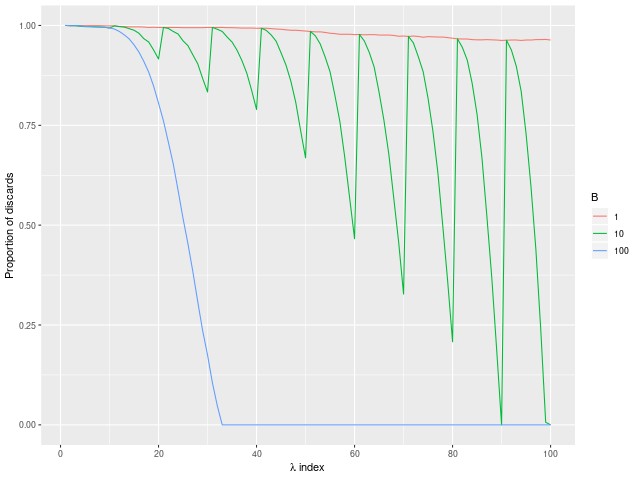
\includegraphics[scale = 0.5]{plots/batchsizes.png}
\end{center}

BEDPP (Basic EDPP) rule is the special case of batched EDPP with only one batch of the largest possible size $B=K=100$. When the batch is large, the safe rule screening will eventually fail to discard any features and make the KKT condition checking cost increase to its maximum $np$. SEDPP rule is the special case where all batches have the smallest possible batch size $B=1$. It remains very powerful along the path, making the KKT condition checking cost almost 0, but the safe screening itself is costly and takes $np$ time per $\lambda$-value. Batched EDPP can strike a balance between BEDPP and SEDPP. In this example, using batches with fixed sizes $B=10$ can reduce the safe screening cost by 90\% compared to SEDPP and reduce the KKT checking cost by 50\% to more than 90\% compared BEDPP.

This example also shows the performance of batch EDPP rule changes along the path of $\lambda$-values. Take the batched EDPP with $B=10$ as an example. For the first batch of 10 $\lambda$-values, the batched EDPP stays powerful even at the end, which means this batch is still exploitable. We may want to extend this batch to reduce average safe screening cost without harming the KKT condition checking cost much. For the last batch however, the screening power is close to 0 for the last few $\lambda$-values, which means this batch becomes useless at this point. Starting a new batch earlier can greatly reduce the KKT condition checking cost with relatively small increase in safe screening cost. Also, the performance of batch EDPP rule also depends on many factors such as the data, the range of $\lambda$-values and spacing between $\lambda$-values. These suggest that starting a new batch after every fixed number of $\lambda$-values cannot not be consistently efficient and we want a method that can automatically determine whether to start a new batch given current performance.

\subsubsection{Adaptive batch starting algorithm}

From previous example, we assume the average cost is a convex function of batch size $B$ which decreases first and then after some optimal value increases again. If we want to minimize the average cost per $\lambda$-value, we need to end the current batch when extending the current batch by 1 $\lambda$-value will increase the average cost. That is, end the current batch at $\lambda_{B-1}$ when $\bar{T}_k(B)>\bar{T}_k(B-1)$. From (13), this condition will be:

\begin{equation}
    (B-1)|\mathcal{S}_B|-\sum_{b=1}^{B-1}|\mathcal{S}_b|>p.
\end{equation}
In practice, we will end the batch at $\lambda_B$ and start at $\lambda_{B+1}$ instead, because evaluating $\mathcal{S}_B$ needs screening at $\lambda_B$ and if we have already done the screening, it would be a waste not to use the screening result.

This batch restarting condition is a greedy condition that only considers the current batch cost. In practice, we cannot know about future batches so this is the most reasonable condition. In fact, it can handle the three most common scenarios well. First, if the screening power stays high, meaning $\mathcal{S}_b$ is small for all $b$, then the left-hand-side of (14) will be small and thus at this point we will extend the current batch to further exploit it. Second, if the screening power has been high for a while but dropped suddenly, meaning $\mathcal{S}_B$ is large but $\mathcal{S}_b$ are mostly small for $b=1,2,...,B-1$, then the left-hand-side of (14) will be large and we will end the useless current batch and start a new batch. Last, if the screening power drops dramatically right after the beginning of the current batch, meaning $\mathcal{S}_b$ are close to $p$ for $b=2,3,...,B$, then the left-hand-side of (14) will be approximately $p-|\mathcal{S}_1|<p$. We will not end the current batch although it becomes useless, because if we did, the next batch would be useless as well.

Combined with Algorithm 2, we will propose the pathwise coordinate descent with adaptive batched safe strong rule screening. After ending a batch, if there are still unsolved $\lambda$-values in the path $\lambda_0,\lambda_1,...,\lambda_K$, we can just start a new batch with the rest unsolved $\lambda$-values and apply the same algorithm.

\begin{algorithm}[H]
    \SetKwInOut{Input}{Input}\SetKwInOut{Output}{Output}\SetKwInOut{Pre}{Pre-compute}\SetKwInOut{Initialize}{Initialize}
    \SetAlgoLined
    \Input{$\{x_j\}_{j=1}^p, \{x_j^Ty\}_{j=1}^p, \hat{\beta}(\lambda_k), r(\lambda_k), \lambda_{k+1},...,\lambda_{K}$}
    \Pre{ $\{x_j^Tr(\lambda_k)\}_{j=1}^p, \{x_j^T\hat{y}(\lambda_k)=x_j^Ty-x_j^Tr(\lambda_k)\}_{j=1}^p, \hat{y}(\lambda_k)=y-r(\lambda_k)$}
    \BlankLine
    $B\xleftarrow{}1$ 
    
    \Repeat{$(B-1)|\mathcal{S}_B|-\sum_{b=1}^{B-1}|\mathcal{S}_{b}|>p$ or $B>K$}{
        Safe Screening: $\mathcal{S}_{k+B}\xleftarrow{}\{j:x_j$ not discarded by batched EDPP rule$\}$.
        
        Strong Screening: $\mathcal{R}_{k+B}\xleftarrow{}\{j\in \mathcal{S}_{k+B}:x_j$ not discarded by batched SSR$\}$.
        
        \Initialize{$\hat{\beta}(\lambda_{k+B})=\hat{\beta}(\lambda_{k+B-1}), r(\lambda_{k+B})=r(\lambda_{k+B-1})$}
        
        \Repeat{Post-convergence check passes}{
            Pathwise coordinate descent in Algorithm 1 with only features in $\mathcal{R}_{k+B}$ and with warm start $\hat{\beta}(\lambda_{k+B}), r(\lambda_{k+B})$, until converge. Save the outputs in $\hat{\beta}(\lambda_{k+B}), r(\lambda_{k+B})$.
            
            Post-convergence check for all $j\in \mathcal{S}_{k+B}\setminus\mathcal{R}_{k+B}$,
            
            \uIf{Post-convergence check does not pass}{
                Add violating features to $\mathcal{R}_{k+B}$\;
            }
        }
        $B\xleftarrow{}B+1$
    }
    \Output{$\{\hat{\beta}(\lambda_{k+b})\}_{b=1}^B, r(\lambda_{k+B}),\lambda_{k+B+1},...,\lambda_K$}
    \caption{Pathwise coordinate descent with adaptive batched safe strong rule screening}
\end{algorithm}

\section{Extension to other lasso type problems}
\label{sec:4}

The structure of the batched safe strong rule is easily extendable to any lasso problems that have corresponding sequential strong rule and sequential safe rule. We are going to derive the extensions to two lasso type problems and show these extensions improve computation efficiency.

\subsection{Batched safe strong rule for sparse logistic regression}

The sparse logistic regression model can be defined as:

\begin{equation}
    \hat{\beta}(\lambda)=\underset{(\beta,\beta_0)\in \mathbb{R}^p\times\mathbb{R}^1}{\mathrm{argmin}}-\frac{1}{n}\sum_{i=1}^n\{y_i\log\pi_i(\beta)+(1-y_i)\log(1-\pi_i(\beta))\}+\lambda||\beta||_1,
\end{equation}
where $\pi(\beta)=\{\pi_i(\beta)\}_{i=1}^n=\{p(y_i=1|x_{i1},x_{i2},...,x_{ip})\}_{i=1}^n=\{e^{\eta_i(\beta)}/(1+e^{\eta_i(\beta)})\}_{i=1}^n$ is the predicted value vector and $\eta(\beta)=X\beta$ is the linear function. $X$ are still the $n\times p$ standardized feature matrix but in this model the $y\in\{0,1\}^n$ is an unstandardized binary response vector. $\beta$ is still the $p\times1$ coefficient vector but we also need a $\beta_0$ as the intercept.

We can use SSR to do the strong rule screening with a small change according to the KKT condition. The residual vector now is $r(\lambda_k)=y-\pi(\hat{\beta}(\lambda_k))$. Then the SSR discards the $j$-th feature at $\lambda_{k+1}$ if (4) holds.

For safe rule screening, instead of EDPP rules, Slores (sparse logistic regression screening rule)\cite{wang2014safe} is used. It was proposed as a one-step rule but we will extend it to a batched rule. Let $\Tilde{y}=2y-1\in\{-1,1\}^n$, $r(\lambda_k)=y-\pi(\hat{\beta}(\lambda_k))$.

\begin{theorem}[Batched Slores]
For the sparse logistic regression model (15), let $\lambda_0:=\max_j|x_j^Ty/n|$, $\Tilde{y}=2y-1\in\{-1,1\}^n$. Suppose we have a sequence of $\lambda$ values $\lambda_0>\lambda_1>...>\lambda_K$. $\forall\theta\in(0,1)^n$, let $x_*=argmax_{x_j}|x_j^Ty/n|$ and

\begin{equation}
    \begin{split}
        g(\theta)&=\frac{1}{n}\sum_{i=1}^n\{\theta_i\log \theta_i+(1-\theta_i)\log(1-\theta_i)\},\\
    \nabla g_i(\theta) &= \frac{1}{n}\log\frac{\theta_i}{1-\theta_i}.
    \end{split}
\end{equation}

Under condition (2) except for standardization for $y$, for any $k=1,2,...,K-1$, assume $\hat{\beta}(\lambda_k)$, $r(\lambda_k)=y-\pi(\hat{\beta}(\lambda_k))$, $\theta(\lambda_k)=\{r_i(\lambda_k)\Tilde{y}_i\}_{i=1}^n$ and $\hat{y}(\lambda_k):=\pi(\hat{\beta}(\lambda_k))$ are known. For some $B$ and any $b$ s.t. $k<k+b\leq k+B\leq K$, let

\begin{equation}
    R(\lambda_{k+b})=\sqrt{\frac{n}{2}\bigg[g\bigg(\frac{\lambda_{k+b}}{\lambda_k}\theta(\lambda_k)\bigg)-g\bigg(\theta(\lambda_k)\bigg)+\bigg(1-\frac{\lambda_{k+b}}{\lambda_k}\bigg)\bigg(\nabla g\big(\theta(\lambda_k)\big)\bigg)^T\theta(\lambda_k)\bigg]},
\end{equation}

$d(\lambda_{k+b})=\sqrt{n}(\lambda_k-\lambda_{k+b})/R(\lambda_{k+b})$. For $\xi = -1,1$ and $j=1,2,...,p$,

\begin{enumerate}
    \item If $-\xi sign(x_*^Ty)x_j^Tx_*\geq nd(\lambda_{k+b})$, then
    
    \begin{equation}
        T_\xi(\lambda_{k+b},x_j;r(\lambda_k))=\sqrt{n}R(\lambda_{k+b})-\xi x_j^Tr(\lambda_k);
    \end{equation}
    
    \item If $-\xi sign(x_*^Ty)x_j^Tx_*< nd(\lambda_{k+b})$, then
    
    \begin{equation}
        T_\xi(\lambda_{k+b},x_j;r(\lambda_k))=R(\lambda_{k+b})\sqrt{n+nu_\xi^2-2\xi u_\xi sign(x_*^Ty)x_j^Tx_*}-nu_\xi(\lambda_k-\lambda_{k+b})-\xi x_j^Tr(\lambda_k),
    \end{equation}
    where
    \begin{align}
        u_\xi&=\frac{-\xi a_1+\sqrt{\Delta}}{2a_2},\\
        a_0&=(x_j^Tx_*)^2-n^2d^2(\lambda_{k+b}),\nonumber\\
        a_1&=-2n\,sign(x_*^Ty)x_j^Tx_*\big(1-d^2(\lambda_{k+b})\big),\nonumber\\
        a_2&=n^2\big(1-d^2(\lambda_{k+b})\big),\nonumber\\
        \Delta&=a_1^2-4a_0a_1.\nonumber
    \end{align}
\end{enumerate}

Then $\hat{\beta}_j(\lambda_{k+b})=0$ if
        \begin{equation}
            \max_{\xi=\pm1} T_\xi(\lambda_{k+b},x_j;r(\lambda_k))
        \end{equation}
\end{theorem}

When computing the batched Slores, $\{x_j^Ty\}_{j=1}^p$ and $\{x_j^Tx_*\}_{j=1}^p$ need to be computed only once, stored and reused for the whole solution path $\lambda_0>\lambda_1>...>\lambda_K$. Other than those two terms, the only term that requires expensive $O(np)$ computation is $\{x_j^Tr(\lambda_k)\}_{j=1}^p$, which only needs to be computed once for each batch. Thus algorithm 3 for adaptive batched safe strong rule can be done with Slores rule instead of EDPP rule to do screening for sparse logistic regression model.

\subsection{Batched safe strong rule for group lasso}

The group lasso problem \cite{yuan2006model} can be defined as:

\begin{equation}
    \hat{\beta}(\lambda) = \underset{\beta\in \mathbb{R}^p}{\mathrm{argmin}}\frac{1}{2n}\bigg|\bigg|y-\sum_{g=1}^GX_g\beta_g\bigg|\bigg|_2^2+\lambda\sum_{g=1}^G\sqrt{p_g}||\beta_g||_1,
\end{equation}
where $\beta=(\beta_1^T,...,\beta_G^T)^T$, $X_g$ is a $n\times p_g$ sub-matrix consisting of columns of $X$ corresponding to features in group $g$, $g=1,2,...,G$. Besides standardization in (2), we apply an addition level of standardization at the group level\cite{breheny2015group}:

\begin{equation}
    X_g^TX_g=nI_{p_g\times p_g},\qquad g=1,2,...,G.
\end{equation}

According to the KKT condition, we can use SSR to do strong rule screening. Given $r(\lambda_k)=y-\sum_{g=1}^GX_g\hat{\beta}_g(\lambda_k)$, we discard features in the $g$-th group at $\lambda_{k+1}$ if:

\begin{equation}
    \bigg|\bigg|\frac{1}{n}X_g^Tr(\lambda_k)\bigg|\bigg|_2<\sqrt{p_g}(2\lambda_{k+1}-\lambda_k).
\end{equation}

For safe rule screening, we have SEDPP for group lasso\cite{wang2013lasso} and we can extend it the batched EDPP rule for group lasso.

\begin{theorem}[Batched EDPP for group lasso]
For the group lasso problem (22), let $\lambda_0:=\max_j\frac{||X_g^Ty||_2}{n\sqrt{p_g}}$. Suppose we have a sequence of $\lambda$ values $\lambda_0>\lambda_1>...>\lambda_K$. Under condition (2) and (23)
    \begin{enumerate}
        \item For any $k=1,2,...,K-1$, given $\hat{\beta}(\lambda_k)$, $r(\lambda_k)$ and $\hat{y}(\lambda_k):=\sum_{g=1}^GX_g\hat{\beta}_g(\lambda_k)$, then for some $B$ and any $b$ s.t. $k<k+b\leq k+B\leq K$, $\hat{\beta}_g(\lambda_{k+b})=0$ if
        \begin{equation}
            \begin{split}
                &\left|\left|2\lambda_{k+b}X_g^Tr(\lambda_k)+(\lambda_k-\lambda_{k+b})\left( X_g^Ty-\frac{y^T\hat{y}(\lambda_k)X_g^T\hat{y}(\lambda_k)}{||\hat{y}(\lambda_k)||_2^2}\right)\right|\right|_2\\
                &<2n\lambda_k\lambda_{k+b}\sqrt{p_g}-(\lambda_k-\lambda_{k+b})\sqrt{n||y||_2^2-\frac{n(y^T\hat{y}(\lambda_k))^2}{||\hat{y}(\lambda_k)||_2^2}}
            \end{split}
        \end{equation}
        \item For k=0, i.e., $\lambda_k=\lambda_0$, let $X_*=argmax_{X_g}\frac{||X_g^Ty||_2}{n\sqrt{p_g}}$ with dimension $n\times p_*$, then for some $B$ and any $b$ s.t. $0<b\leq B\leq K$, $\hat{\beta}_g(\lambda_{k+b})=0$ if
        \begin{equation}
        \left|\left|(\lambda_0+\lambda_b)X_g^Ty-(\lambda_0-\lambda_b)X_g^TX_*X_*^Ty\right|\right|_2<2n\lambda_0\lambda_b\sqrt{p_g}-(\lambda_0-\lambda_b)\sqrt{n||y||_2^2-n^2\lambda_0^2p_*}.
    \end{equation}
    \end{enumerate}
\end{theorem}

Similar to Batched EDPP rule, three expensive computations are $\{X_g^Ty\}_{g=1}^G$, $\{X_g^TX_*\}_{g=1}^G$ and $\{X_g^Tr(\lambda_k)\}_{g=1}^G$. The first and second only need to be computed once for the whole solution path. The last only needs to be computed once per batch with cost $O(np)$.

\section{Experiments}
\label{sec:5}

\subsection{Simulations}
\label{sec:sim}
\begin{itemize}
    \item Introduction to biglasso package
\end{itemize}
\begin{itemize}
    \item Comparing active set cycling, strong rules, SEDPP, Hybrid SSR, and proposed Batched SSR
    \item Varying n, p. Computation time for all methods grow linearly and ratios among them are constant.
    \item Varying signal-noise ratio. As the signal increases, the proposed method has larger advantage over other method.
    \item Varying $||\beta||_0$, number of non-zero coefficients, or sparsity. When the model is sparser, the proposed method has larger advantage over other methods.
\end{itemize}

\subsection{Real data analysis}
\label{sec:real-data}

\subsection{Big data performance}

\begin{itemize}
    \item Analyse and profile different methods. Compare them in big data case ?
\end{itemize}

\section{Conclusion}
\label{sec:6}


\bibliographystyle{unsrt}
\bibliography{ref}

\end{document}
